
\fullcite{hard91}

%-------------------
\begin{multicols}{2}
\begin{center}
{\bf Article excerpts}
\\ 
{\bf Notes and remarks}
\end{center}
\end{multicols}


\begin{multicols}{2}
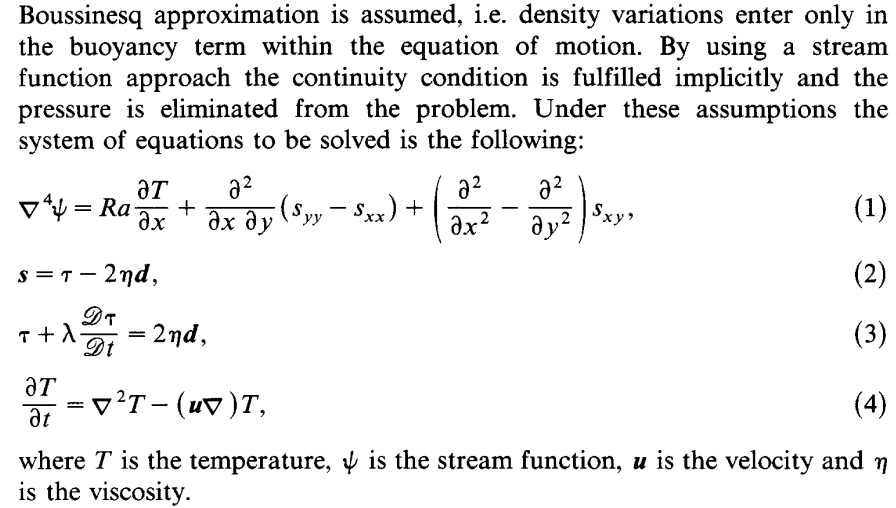
\includegraphics[width=8.3cm]{images/viscoelasticity/hard91_a}\\
What is ${\bm s}$ here? it is defined as "non-Newtonian 
contribution to the stress tensor ${\bm\tau}$.
\[
\frac{{\bm \tau}}{2\eta} + \frac{\lambda}{2\eta}\frac{{\cal D}{\bm \tau}}{{\cal D}t}
=\dot{\bm\varepsilon}
\]
Probably here $\lambda=\eta/\mu$ (see \ref{ve_momy93}), so that 
\[
\frac{{\bm \tau}}{2\eta} + \frac{1}{2\mu}\frac{{\cal D}{\bm \tau}}{{\cal D}t}
=\dot{\bm\varepsilon}
\]
\end{multicols}

\begin{multicols}{2}
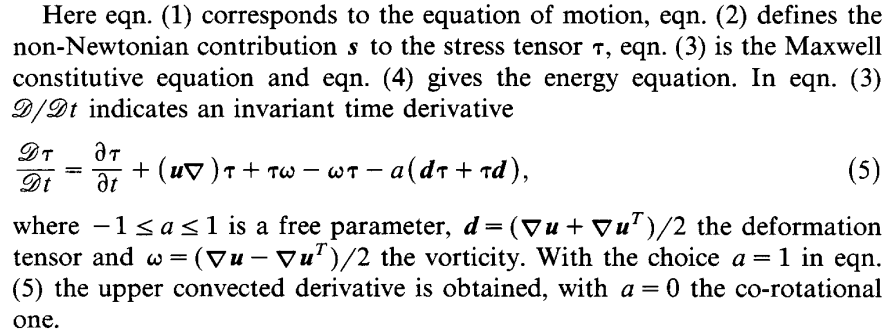
\includegraphics[width=8.3cm]{images/viscoelasticity/hard91_b}\\
\[
\frac{{\cal D}{\bm \tau}}{{\cal D}t}
=
\frac{\partial {\bm \tau}}{\partial t}
+(\vec\upnu\cdot \vec\nabla) {\bm \tau}
+ {\bm \tau}\cdot \dot{\bm\omega} - \dot{\bm \omega}\cdot {\bm \tau}
- a (\dot{\bm\varepsilon} \cdot {\bm \tau} + {\bm \tau}\cdot \dot{\bm\varepsilon})
\]
\end{multicols}

\begin{multicols}{2}
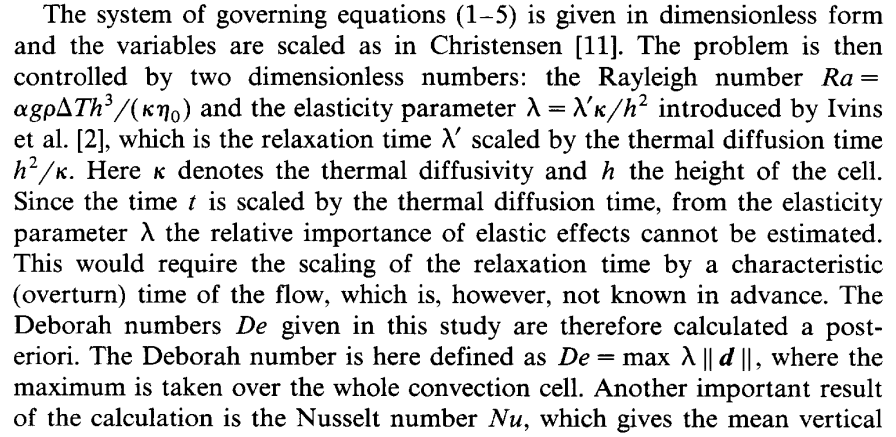
\includegraphics[width=8.3cm]{images/viscoelasticity/hard91_c}\\
\end{multicols}
